\section{Architectural design}

\subsection{Overview}
	\subsubsection{Context viewpoint}
	
		\begin{figure}[h]
			\centering
			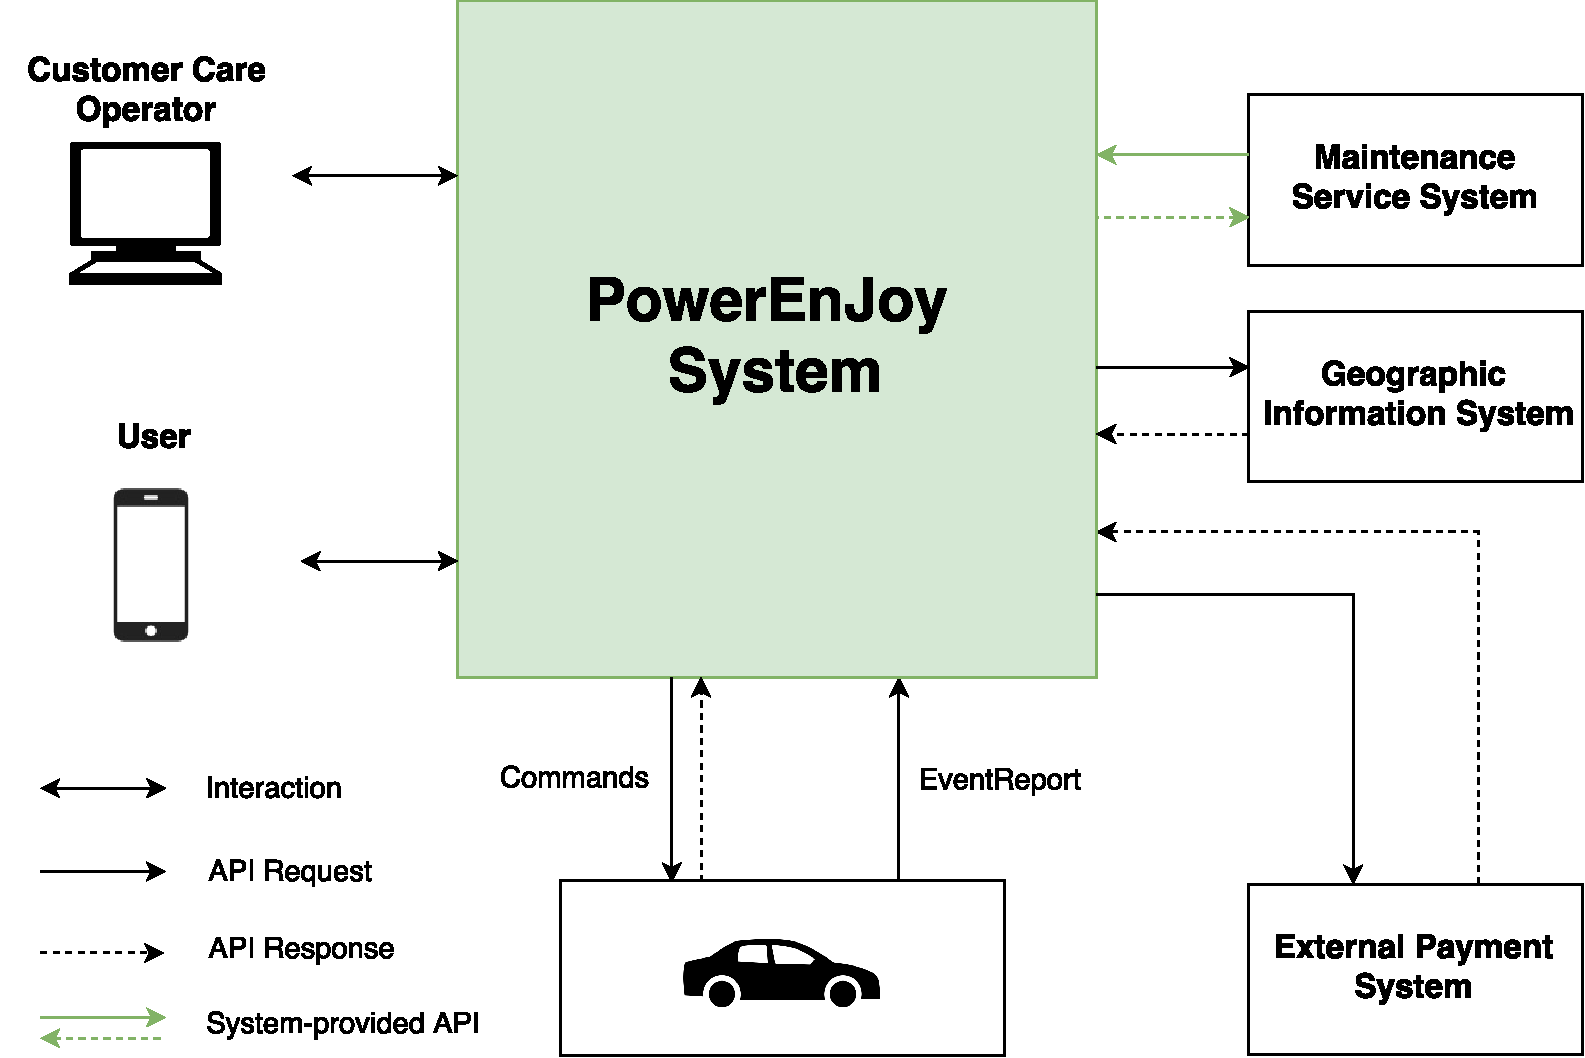
\includegraphics[width=\linewidth]{contextViewPoint}
			\caption{
				\label{fig:contextViewPoint} 
				Context viewpoint
			}
		\end{figure}
		
		We need to design a system which allows communications with many agents such as cars, users, external systems, etc.
		Moreover we recognize that in most of the interactions the system is providing a service to agents so, after taking in consideration different alternatives, we decided to use a client-server architectural approach.

		\begin{figure}[h]
			\centering
			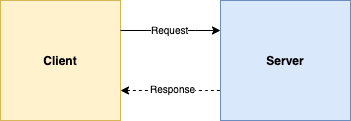
\includegraphics[width=0.5\linewidth]{ClientServer}
			\caption{
				\label{fig:ClientServer} 
				Client Server architecture
			}
		\end{figure}
		
		Cars offer to the system a set of primitives which allow it to interact with them: in this case it is clear that cars are providing the system services, so they can be identified as servers while the system acts as a client; on the other end the notification functionality offered by cars clearly yields to an event-based approach due to the asynchronous nature of such interactions, this led us to use a publish-subscribe paradigm for these specific interactions.
		\clearpage
		
		
		
	\subsubsection{Composition viewpoint}
	
		\begin{figure}[h]
			\centering
			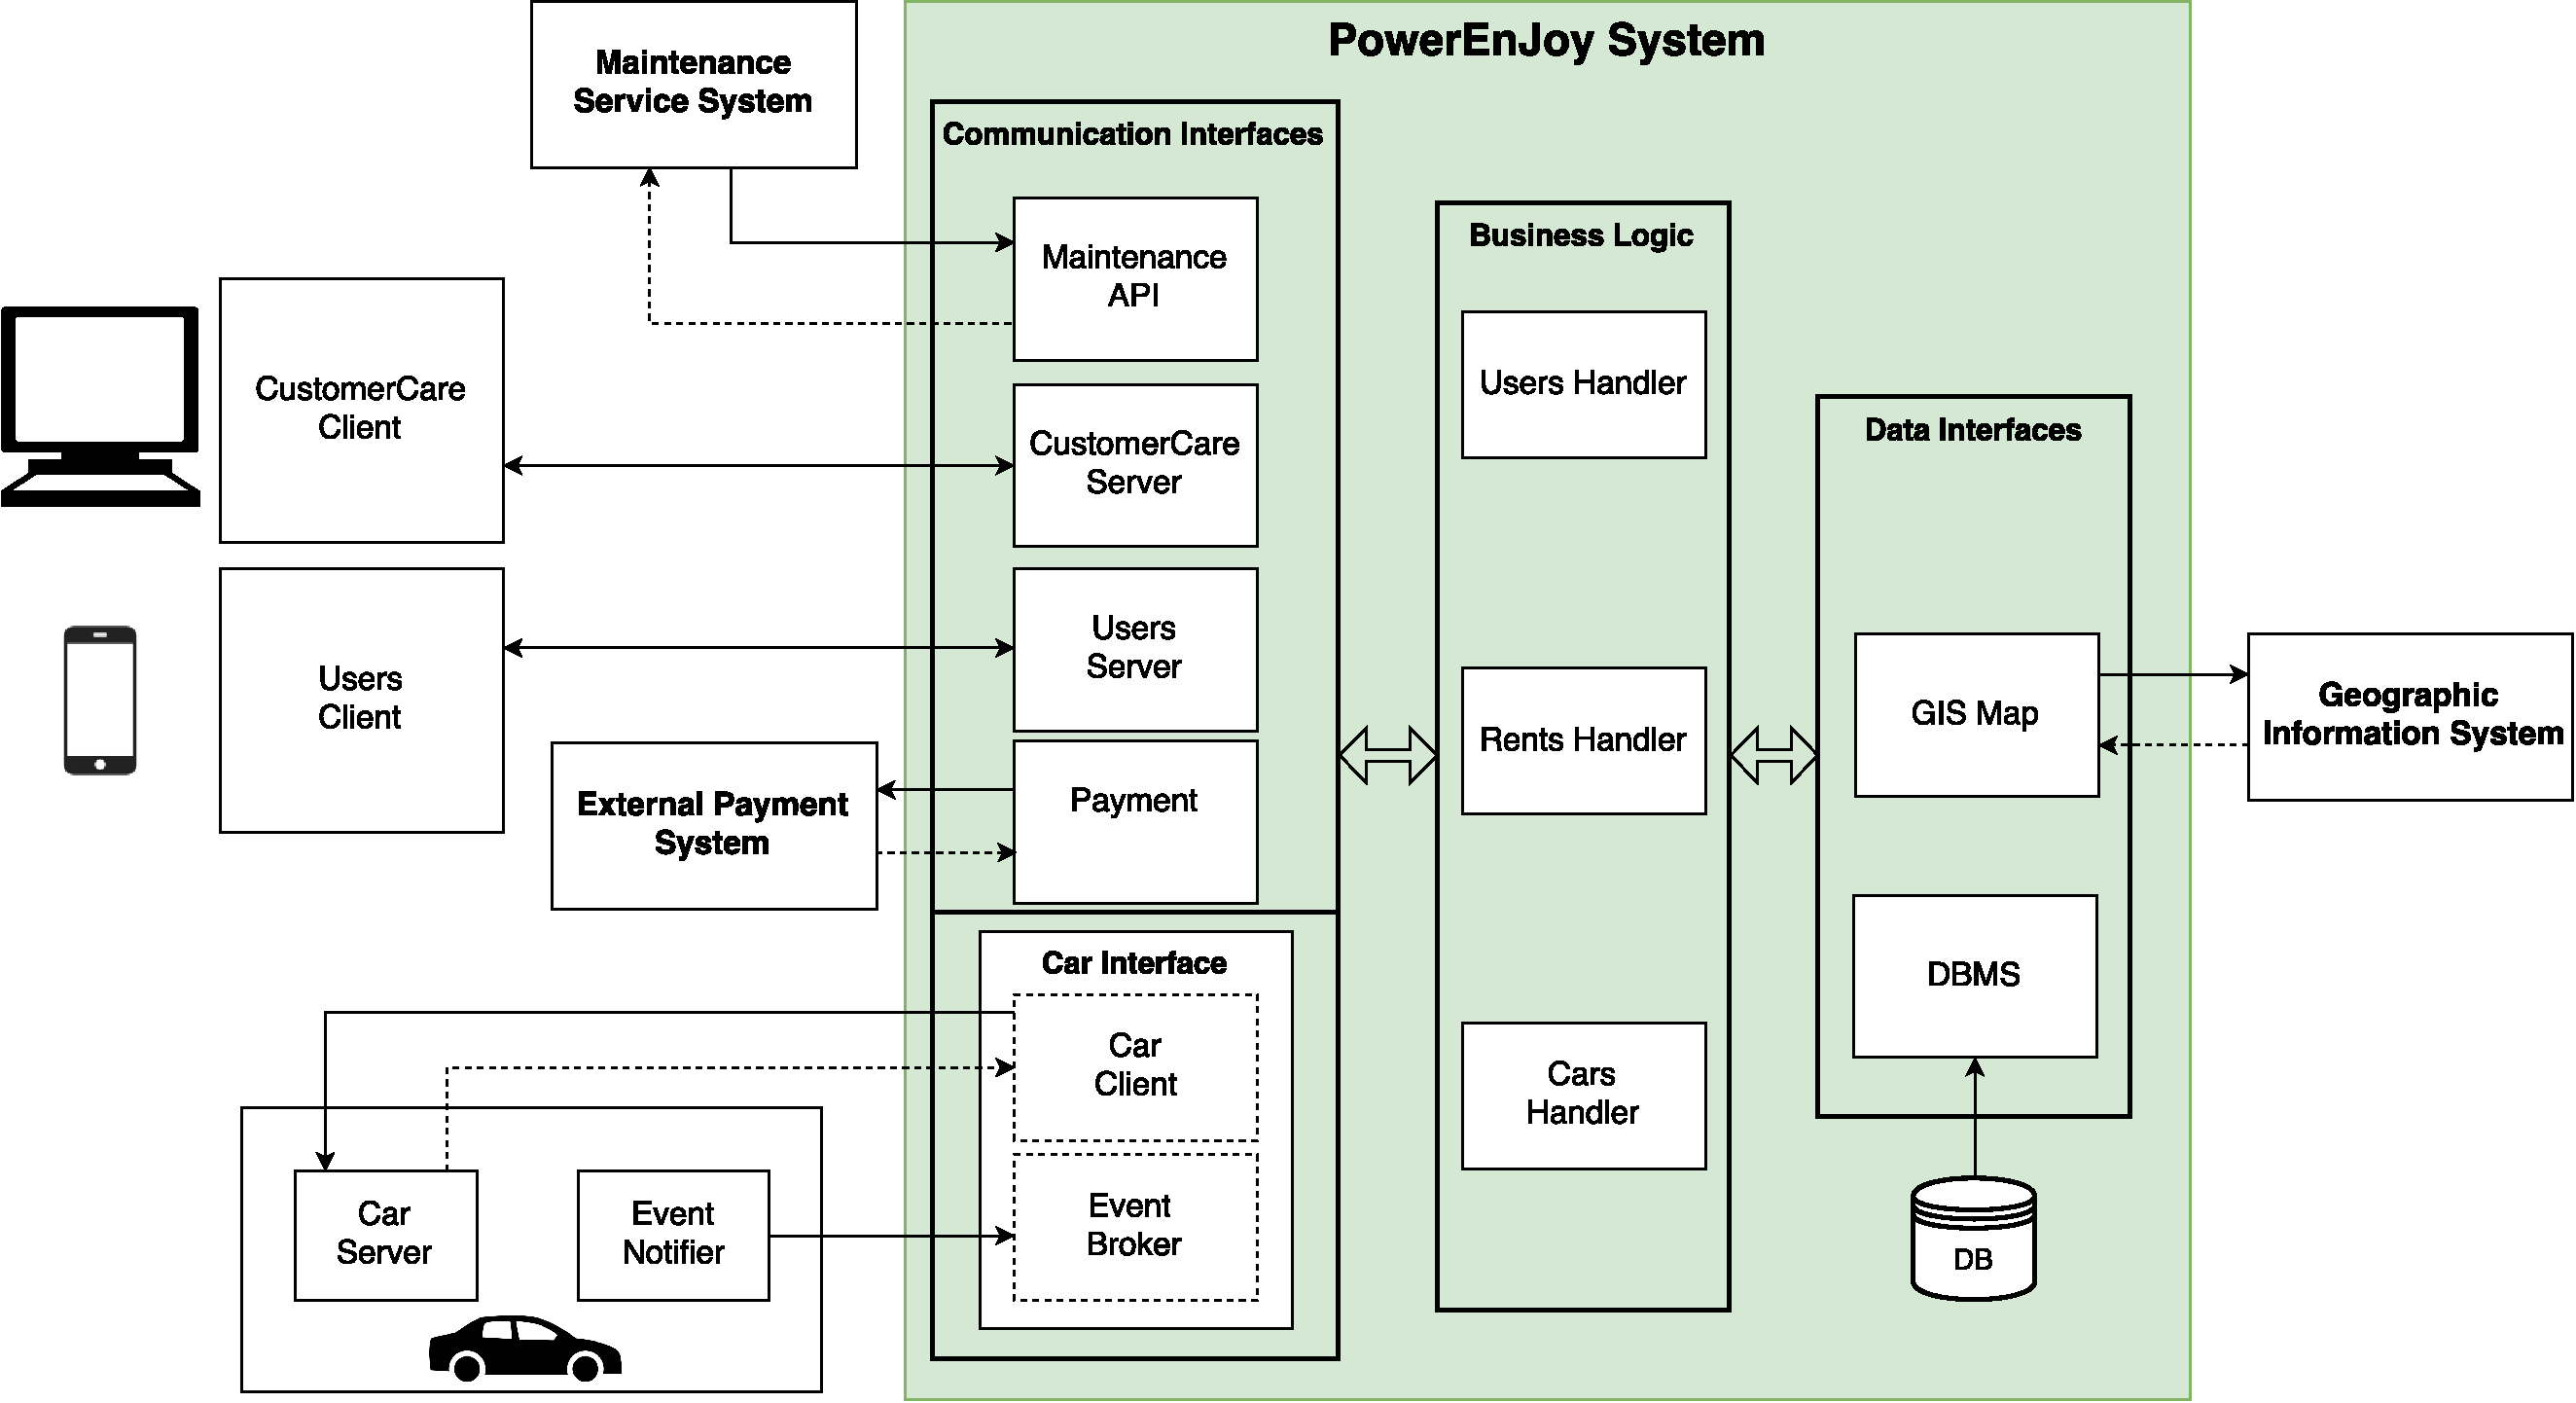
\includegraphics[width=\linewidth]{ComponentOverview}
			\caption{
				\label{fig:compositionViewPoint} 
				Composition viewpoint
			}
		\end{figure}
		
		Going deeper in the analysis of our system composition, we are able to identify some of the modules that will be required in order to provide the functionalities specified in the Requirement Analysis and Specification Document. 
		\paragraph{Communication Interfaces}
			Since our system interacts with many external agents, it needs to have different \emph{Communication Interfaces} in order to communicate with them. 
		\begin{itemize}
			\item An API is needed to provide \emph{Maintenance Service System} the information it needs to work with us
			\item A software module is needed in order to provide users functionalities of the system 
			\item A software module is needed to provide the \emph{Customer Care} the functionalities it needs
			\item An internal payment software module will deal with the communication with the \emph{External Payment System} 
			\item A set of modules will manage the communications between the cars and the system: a module to call primitives on cars through the provided API and another one to observe events triggered by the car. When the trigger method is called on \emph{CarClient}, it enables the requested triggers on the car passed as a parameter. This allows the cars to notify to the system the events related to the aforementioned triggers; these events will be received and dispatched by the \emph{EventBroker} to the subscribed components.
		\end{itemize}
\clearpage
\begin{figure}[h]
	\centering
	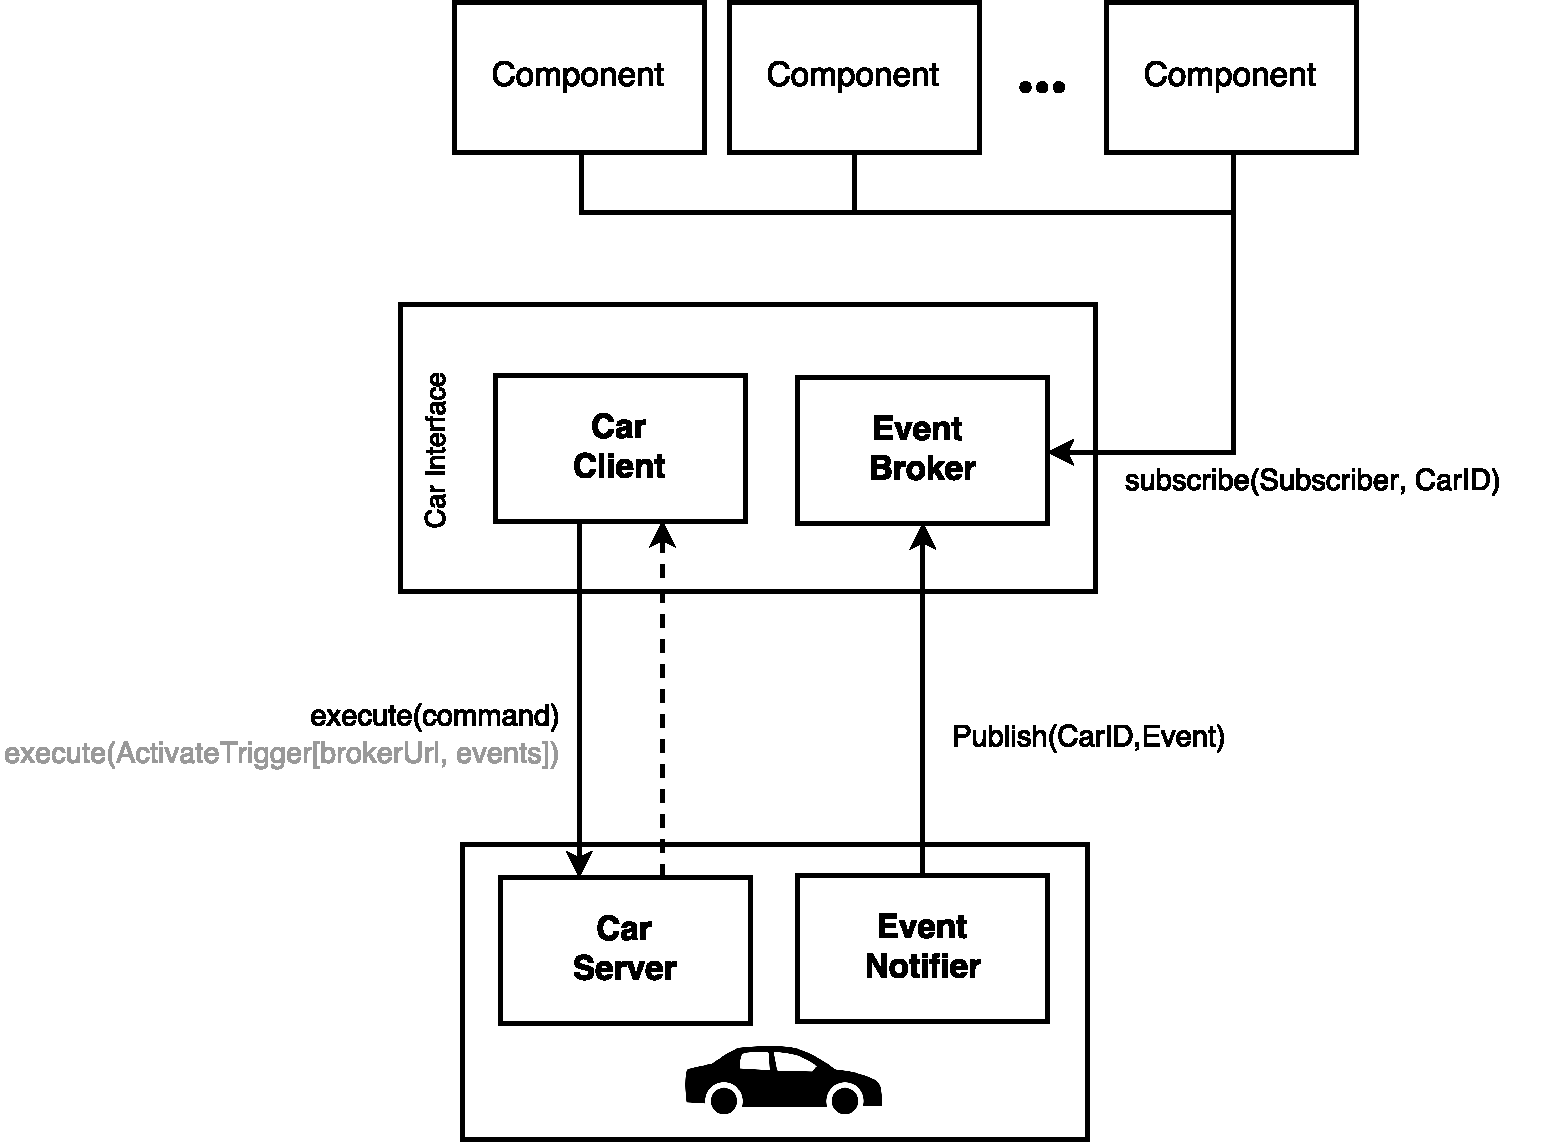
\includegraphics[width=\linewidth]{carInterface}
	\caption{
		\label{fig:carInterface} 
		Car communication Interface
	}
\end{figure}


		\paragraph{Business Logic}
			The actual application logic of our system needs to manage the users information, the rents and the cars information; for each of these purposes several software modules are necessary; they will use communication interfaces to communicate with the agents and they will be able to retrieve data from the data interfaces.
		\paragraph{Data Interface}
			Our system needs a way to access and store the data it produces or retrieves from external resources, that is why \emph{Data Interface} modules are needed. These modules allows interaction between the \emph{Business Logic} modules and the System Databases; moreover they provide an interface to communicate with the GIS in order to allow the \emph{Business Logic} modules to access its functionalities.

\clearpage
\subsection{Component view}
\begin{figure}[h]
	\centering
	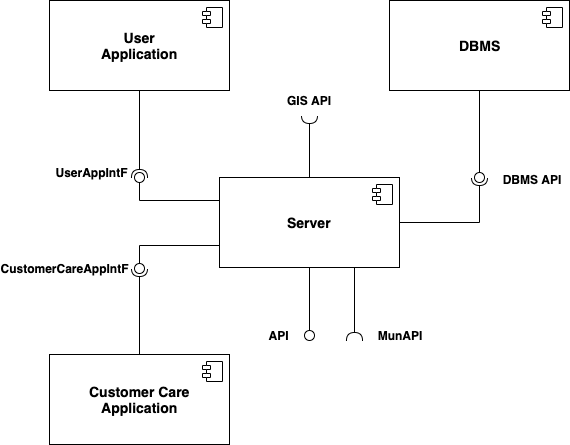
\includegraphics[width=\linewidth]{highLevelComponents}
	\caption{
		\label{fig:highLevelComponents} 
		High-level components
	}
\end{figure}

\subsection{Deployment view}

\subsubsection{Four tier architecture}
Taking into account that:
\begin{itemize}
	\item the \emph{Composition viewpoint} diagram shows the need of database decoupling from the actual system
	\item in the \emph{Server component view} we can clearly distinguish modules who take care of presentation and communication with the client
	\item in the \emph{Server component view} we can clearly distinguish modules who take care of the specific application logic
\end{itemize}
we decided to design the system on a four tier architecture pattern (see also \label{sec:deploymentView}
\begin{figure}[h!]
	\centering
	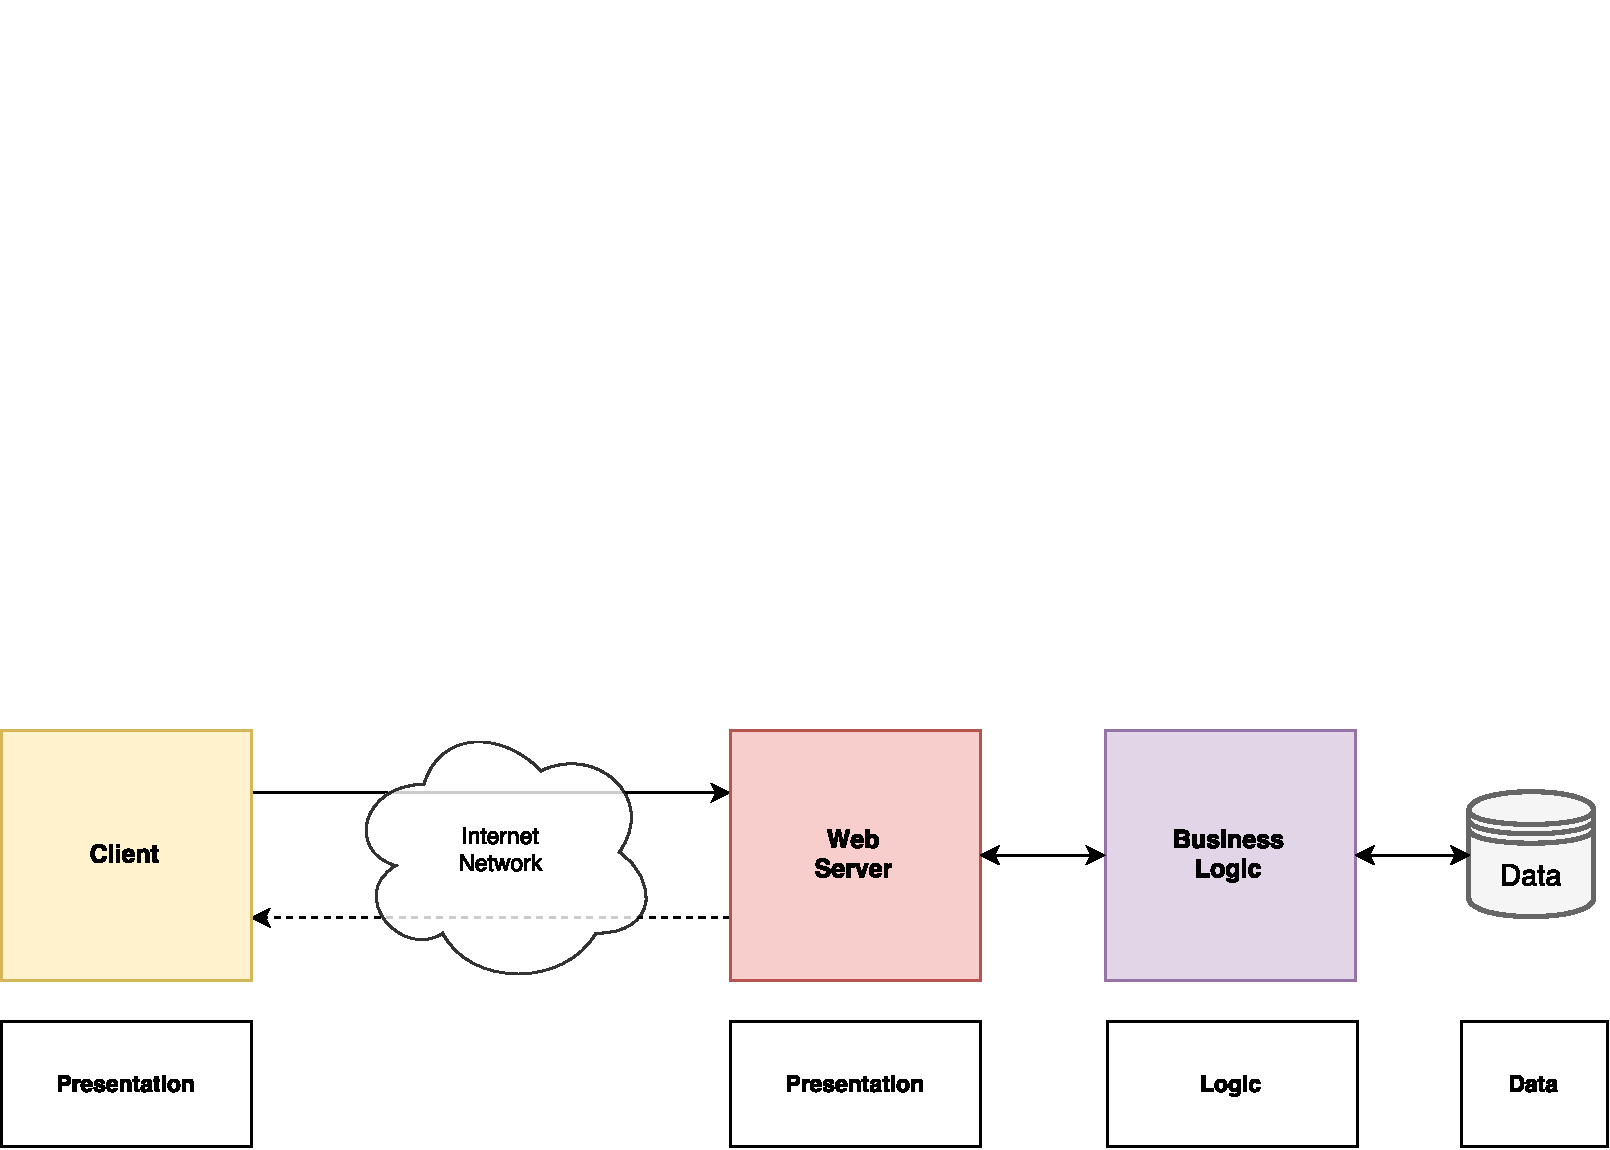
\includegraphics[width=\linewidth]{4Tier}
	\caption{
		\label{fig:fourTierCloud} 
		Four tier architecture with internet layer
	}
\end{figure}
\paragraph{Mapping of Server components on architecture:}to clarify at a finer level how the Server components are mapped in the four tier layered architecture the following diagram represents the Server components highlighted in the same color of the tier in the previous diagram:
\begin{itemize}
	\item Client: components used by users in order to access the functionalities offered by the system
		\begin{itemize}
			\item UserApplication
			\item CustomerCareApplication
		\end{itemize}
	\item Web Server: components which provides interfaces to clients in order to allow them to use functionalities offered by the system
		\begin{itemize}
			\item UserAppServer
			\item CustomerCareServer
		\end{itemize}
	\item Business Logic: components which realizes the functionalities offered by the system
		\begin{itemize}
			\item RentManager
			\item AccessManager
			\item UserInformationManager
			\item MaintenanceManager
			\item EventBroker
			\item CarHandler
			\item DataProvider
		\end{itemize}
	\item Data: components which store and manage the access to the data produced and needed by the Business Logic
		\begin{itemize}
			\item DBMS
		\end{itemize}
\end{itemize}

\begin{figure}[h]
			\centering
			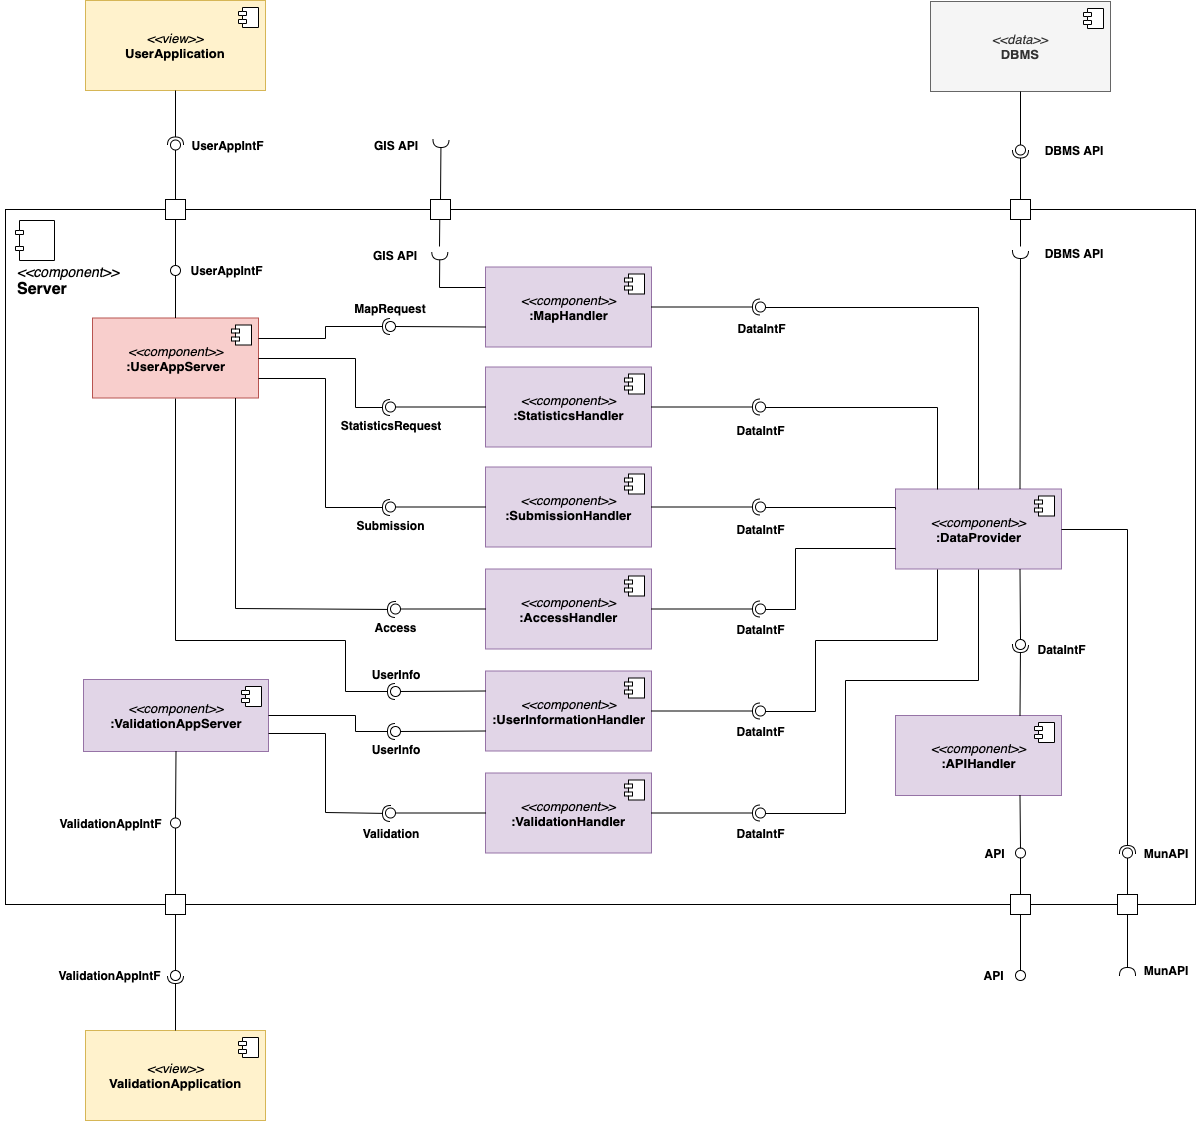
\includegraphics[angle=90,width=0.9685\linewidth]{deployComponent}
			\caption{
				\label{fig:deployServerComponent} 
				Mapping server component on architecture
			}
		\end{figure}
\clearpage

\subsubsection{Deployment diagram}
The diagram in \autoref{fig:deployment} represents the mapping of the software components depicted in \autoref{fig:deployServerComponent} and \autoref{fig:highLevelComponents} on the devices that will run them. Many design concerns were considered while developing this solution.
\paragraph{Security:}security is ensured in different points of the architecture, in particular the \emph{UserAppServer} uses HTTPS as communication protocol to communicate with the users; the devices running the \emph{CustomerCareApplication} component are in a VPN with the device running the \emph{CustomerCareServer}.
\paragraph{Scalability:}this model of deployment is scalable in the sense that the system administrators will be able to add more devices and deploy more instances of the needed components when and where performance issues will arise, in order to maintain a minimum level of performance even with loads increase.
\paragraph{Decoupling:}decoupling in this architecture is present at different levels; in the deployment diagram it is clear that the each of the four tier runs on different devices, moreover the \emph{UserAppServer} component runs on a different device than the \emph{CustomerCareServer}, the Maintenance API and the \textit{CarEventHandlerIntF} interface.
\paragraph{Redundancy:}in this iteration of the architecture no redundancy of components or devices is present, but it is allowed in prevision of future expansions of the system's infrastructure.
\paragraph{Fault Tolerance:}deploying different components on different machines allows the system to be easier to recover in case of a problem on one of the machines; for an example the Web Server running the \textit{UserAppServer} component goes down, it can be replaced with another machine and in the mean time the \textit{ApplicationServer} would still be up and running and still be able to provide the \textit{CustomerCareApplication} with its functionalities.
\clearpage

\begin{figure}[t!]
	\centering
	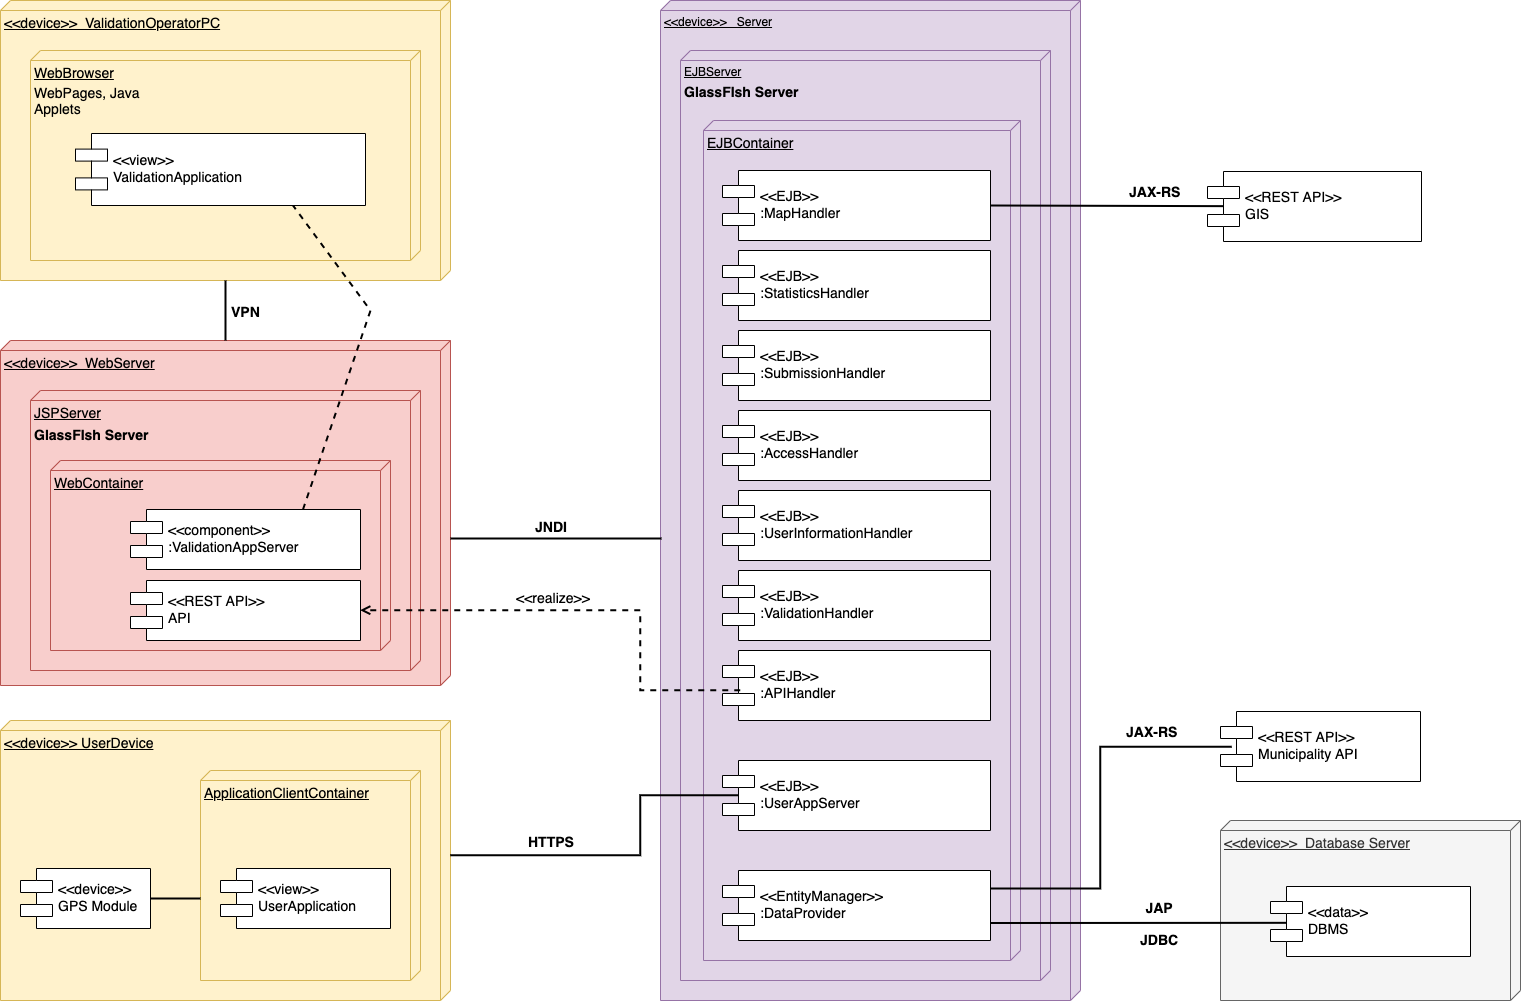
\includegraphics[width=\linewidth]{deployment}
	\caption{
		\label{fig:deployment} 
		Deployment diagram
	}
\end{figure}

\clearpage
\subsection{Runtime view}
In this section we represent some runtime views of the supposed interactions between the components of the \emph{PowerEnJoy} system.

\paragraph{Notes to read the diagram} When an attribute is modified in a JPA object the changes are reflected into the \emph{DataProviderComponent} in order to keep the database updated.

\clearpage
\subsection{Component interfaces}
